\begin{multicols}{3}[\section{Iridium}]

\rhead{Benita Rojewski}
\lfoot{08.05.2016}

\newrefsegment

\begin{tabular}{p{2,1 cm}p{2.7 cm}}
\textbf{Steckbrief}& \\
\end{tabular}
\rowcolors{1}{\topicolor!20}{}
\begin{tabular}{p{2,1 cm}p{2.7 cm}}
      Einsatz seit & September 1998\\
      Vorwahl & +8816 und +8817\\
      Frequenz"-bereich  & L-Band:
      \SI{1616}bis\SI{1626.5}{\mega\hertz}, 
      K-Band: \SI{19.4} bis\SI{19.6} {\giga\hertz}, \SI{29.1} bis \SI{29.3} {\giga\hertz}\\
      Datenrate (komprimiert) & \SI{26} bis \SI{27} {bit/s}\\
      Datenrate (unkomprimiert) & \SI{2.4} bis \SI{2.5} {bit/s}\\
      Verbreitung & Weltweit, Iridium Satellite and Network Operations Center \\
      Modulation & FDMA, TDMA\\
      Sendeleistung (während des Sendens) & max. 7 Watt\\
      Sendeleistung (während des Empfangs) & 0.6 Watt\\
      Verschlüsselung/ Kodierung & „Advanced Multi-Band Excitation“ (AMBE)\\
      Schutzart & IP54\\
      Dual Play & Ja\\
      Triple Play & Nein\\
\end{tabular}
\par
%Source http://www.fh-bingen.de/fileadmin/user_upload/Lehrende/Kilsch_Dieter/internet/projekte/TedoSchStiUnits.pdf -> Seite 9 findet ihr alle verwendbaren Einheiten, wie:
%\SI{Zahl}{\mega\hertz} oder \SI{Zahl}{\mili\metre}
%Ich weiß ehrlich gesagt nicht welche Einheiten ihr im Text genau braucht, aber in dem Dokument und mit obigen Beispiel sollte es umsetzbar ein.
\subsection*{Überblick}

In der Kommunikationstechnik ist Iridium der Name für ein drahtloses Kommunikationsnetz. Dieses besteht aus 68 Satelliten, von denen zwei Reserve sind. Sie befinden sich in einer Höhe von  780 km in sechs nahezu polaren Umlaufbahnen mit je elf sich im aktiven Einsatz befindenden Satelliten und einem Reservesatelliten je Bahn. Somit liegen diese in erdnaher Umlaufbahn. Dadurch ist es gewährleistet, dass Signale von einem Mobiltelefon gesendet und empfangen werden können (siehe Abb. \ref{fig:sv}).
Da ursprünglich dieses System aus 77 Satelliten bestehen sollte, hat es den Namen Iridium erhalten. Dieses Element hat im Periodensystem die Ordnungszahl 77.\cite{I3,I5}

\begin{Figure}
	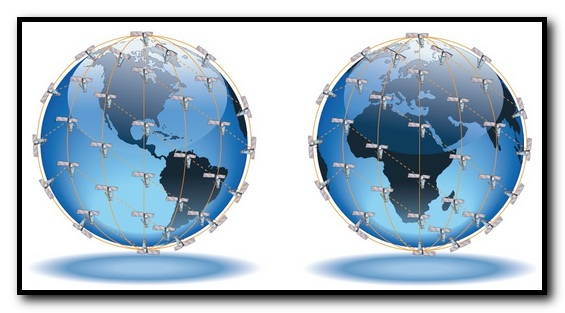
\includegraphics[width=\linewidth]{Kapitel/Iridium/Grafiken/satellitenverteilung.jpg}
	\captionof{figure}{Satellitenverteilung~\cite{I6}}
	\label{fig:sv}
\end{Figure}


\subsection*{Technische Erläuterung}
Die Verknüpfung der Iridium-Satelliten ist netzförmig und mit den Iridium-Gateways weltweit verbunden. Erst dadurch entsteht die Möglichkeit,mit den öffentlichen Telefon- und Mobil-funknetzen in Kontakt zu treten.
Zudem sind die Satelliten des Iridium-Netzwerks untereinander durch Intersatellitenlinks verbunden. 

Eine aktive Verbindung kommt zustande, wenn sich ein Satellit in Reichweite einer Vermittlungsstelle auf der Erdoberfläche befindet. Dadurch entsteht der Weg in das uns bekannte Telefonnetz. Besteht keine Verbindung von den Satelliten zur Empfangsstation, so werden die Telefongespräche oder auch Signale über andere Iridium-Satelliten weitergeleitet, bis es zu einer Kontaktaufnahme mit einem Empfangssatelliten kommt.

Im \textbf{L}(ong)-Band werden die Daten vom Satelliten zum Endgerät übertragen. Die Übertragung zwischen den Satelliten und von diesen zur Empfangsstation erfolgt im \textbf{Ka}(y-ay)-Band. In Abbildung \ref{fig:Fs} ist das Frequenzspektrum des Iridium-Systems mit der jeweiligen Aufgabe dargestellt: 

\begin{Figure}
	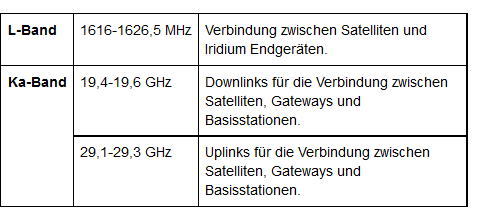
\includegraphics[width=\linewidth]{Kapitel/Iridium/Grafiken/band.png}
	\captionof{figure}{Frequenzspektrum des Iridium-Systems~\cite{I1}}
	\label{fig:Fs}
\end{Figure}

Kommunizieren zwei Iridium-Nutzer  miteinander, so wird dieses Gespräch direkt zwischen den Satelliten vermittelt, ohne eine Erdstation dazwischen zu schalten. ~\cite{I1, I4}



\subsubsection*{Netzabdeckung}
Voraussetzung für die Iridium-Kommunikation ist eine klare Sicht zum Himmel in alle Richtungen ab einem Höhenwinkel von 8.2 Grad. Befindet sich jedoch ein Objekt ab diesem Winkel am Himmel, so wird die Kommunikation gestört bzw. unterbrochen. Deshalb wird als Maßstab hierfür die geballte Faust bei waagrecht ausgestrecktem Arm verwendet. Diese Höhe entspricht ungefähr diesem Höhenwinkel. Damit ergibt sich folgende  Netzabdeckung unter dem Höhenwinkel von 8.2 Grad (siehe Abb. \ref{na8.2}).

In Gegenden, in denen tiefe Schluchten oder Bergtäler sind, kann es häufig zu Verbindungsunterbrechungen kommen, so dass es sein kann, dass erst 120 Minuten später wieder eine Verbindung zustande kommt. Grund hierfür ist, dass in diesen zwei Stunden kein Iridium- Satellit in Sichtkontakt kommt.
Die Abbildung \ref{na21} zeigt die Netzabdeckung unter dem Höhenwinkel von 21 Grad in tiefen Schluchten 
\begin{Figure}
	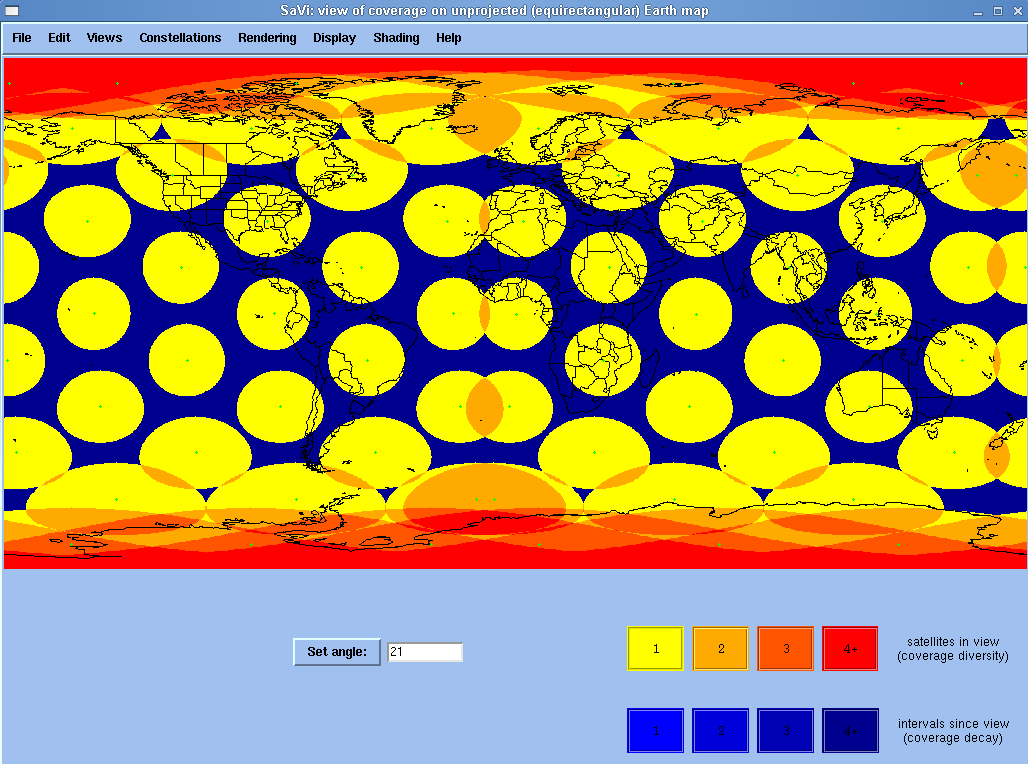
\includegraphics[width=\linewidth]{Kapitel/Iridium/Grafiken/netzabdeckung21.png}
	\captionof{figure}{Netzabdeckung unter dem Höhenwinkel von 21 Grad in tiefen Schluchten ~\cite{I4}}
	\label{na21}
\end{Figure}

Mit Hilfe von Iridium- Satelliten ist es auch möglich, die Polregionen abzudecken. Der Grund hierfür liegt darin, dass auch auf der polaren Umlaufbahn Satelliten platziert sind, so dass dort die Versorgungsdichte besonders hoch ist, da eine geringere freie Sicht zum Himmel als am Äquator benötigt wird.

\begin{Figure}
	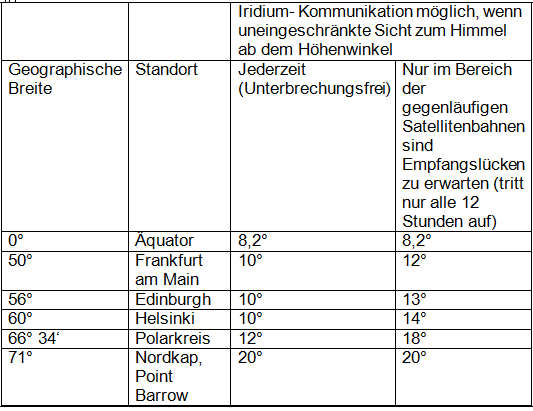
\includegraphics[width=\linewidth]{Kapitel/Iridium/Grafiken/hoehenwinkel.png}
	\captionof{figure}{Höhenwinkel~\cite{I4}}
	\label{fig:hw}
\end{Figure}

Im Durchschnitt findet alle neun Minuten während eines Telefonats ein automatischer Wechsel der Iridium-Satelliten statt, da der verwendetet Satellit hinter dem Horizont verschwindet. Diesen Wechsel bemerken die Gesprächsteilnehmer nur, wenn der alte Satellit hinter dem Horizont verschwindet und der neue Satellit noch nicht in Sichtweite ist.~\cite{I4}

\subsection*{Einsatz}
Vorteil von Iridium ist die Erreichbarkeit in Bereichen mit wenigen Basisstationen, schlechter Verbindung, in freier Natur und in unwegsamen Gelände, die so gut wie immer gegeben ist.
Einige Bereiche, in denen diese Technologie angewendet wird: 

\begin{itemize}
	\item SMS
	\item Militär
	\item Paging
	\item Email
	\item Gas- und Ölgesellschaften
	\item Baugesellschaften
	\end{itemize}

Allerdings kann es auch vorkommen, dass die Frequenzen belegt sind oder die dortige Regierung die Verwendung von Iridium nicht genehmigt, wodurch dann die Kommunikation eingeschränkt ist. Seit 2015 besteht dieses Problem z.B. in den Ländern Kuba und Nordkorea. In Russland und Indien dagegen ist der Import, Export und die Verwendung von Iridium-Satelliten erlaubt, allerdings besteht eine Meldepflicht für solche Art von Telefonen.~\cite{I3,I4}

\subsection*{Anbieter und Gremien}

Für die Satellitensteuerung und die Netzverwaltung ist das \textit{Iridium \textbf{S}atellite and \textbf{N}etwork \textbf{O}perations \textbf{C}enter} (SNOC) zuständig. Ihr Sitz ist im Norden des US-Bundesstaates Virginia. Zudem gibt es Kontrollstellen, die für Telemetrie und Funkpeilung (TTAC) zuständig sind. Diese befinden sich auf Hawaii und in Kanada.

Es kommt durch die Kooperation von vielen nationalen und internationalen Mobilfunknetzen zu Roaming-Partnern, weswegen der Iridium-Kunde über diese seine Telefongespräche führt und damit verschiedene Netze, wie z.B. GSM, AMPS und CDMA, weltweit zu nutzen. Befinden sich die Kunden außerhalb der Versorgungsbereiche der lokalen Mobilfunknetze, so kommen die Satellitennetze zum Einsatz. ~\cite{I1}



\end{multicols}
\newpage
\section*{Historische Entwicklung}
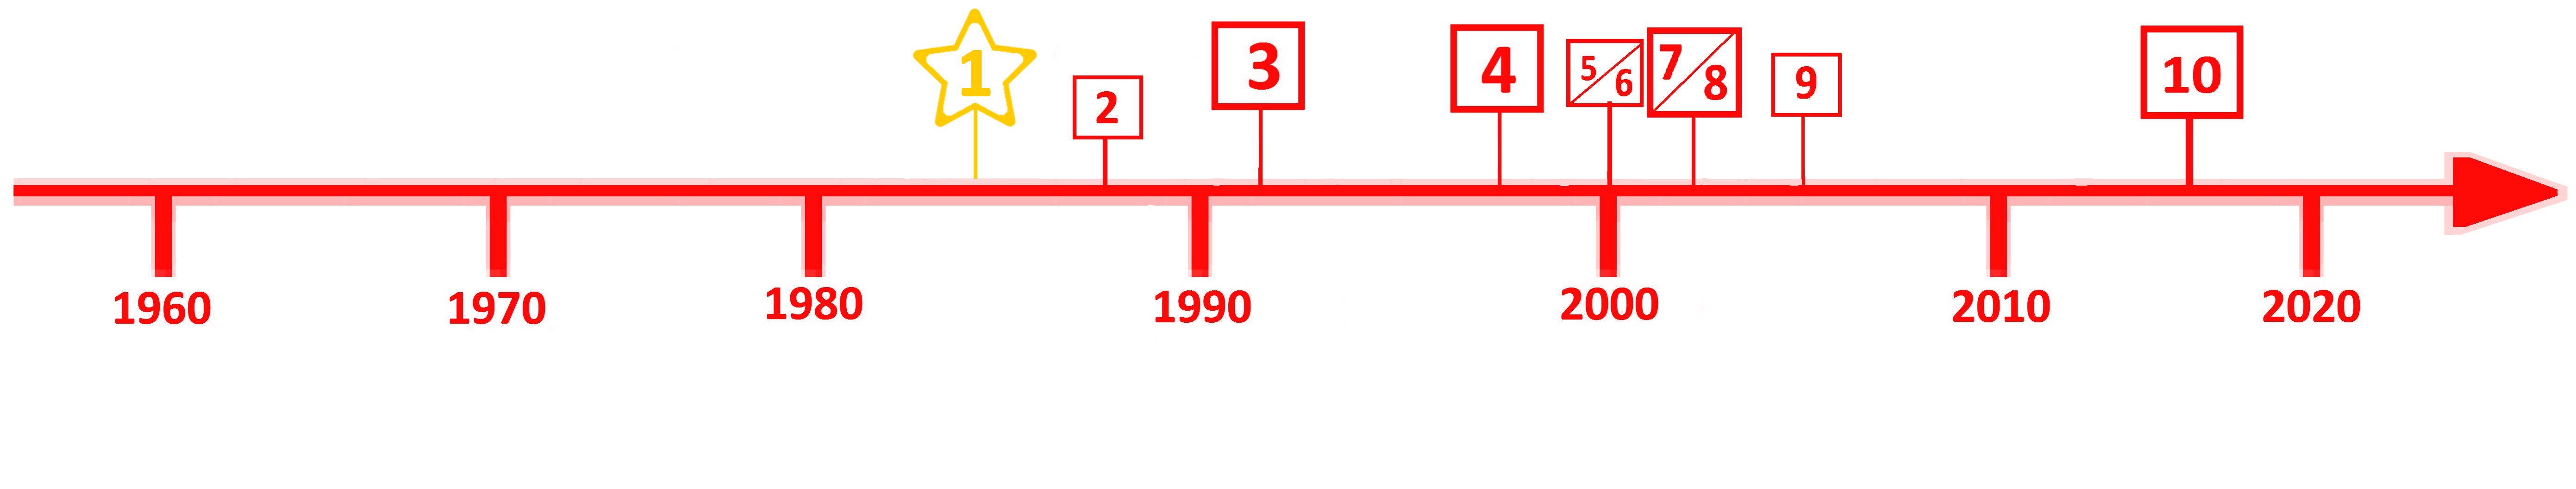
\includegraphics[width=\textwidth]{Kapitel/Iridium/Grafiken/Zeitstrahl_Iridium_rot}
\par
\noindent
\rowcolors{2}{}{\topicolor!20}
\begin{tabular}{p{0.5 cm}p{1.5 cm}p{15.55 cm}}
	Nr. & Datum & Entwicklungsschritte~\cite{I2},~\cite{I4}\\
	1 & 1985 & Geburt der Idee für Iridium bei \textit{Motorola}. Es sollte die weltweite Sprach- und Datenübermittlung über Satellitentelefon und \textbf{PDA}s (\textbf{P}ersonal \textbf{D}igital \textbf{A}ssistant) ermöglichen.\\
	2 & bis 1988 & Konzeptentwurf\\
	3 & 1991 & Gründung des Unternehmens \textit{Iridium Inc}.\\
	4 & 1998  & In Betriebnahme des Systems 
	\\
	5& März 2000 & geplante Abschaltung, allerdings wurde diese auf Grund des Druckes der Öffentlichkeit zum Teil verschoben.\\
	6 & 23.08.2000 & Konkursanmeldung des Unternehmens\\
	7 & 01.01.2001 & Übernahme des neugegründeten Unternehmens \textit{Satellite LLCt}, Betriebnahmen und Wartung der Satelliten von \textit{Boening}, Hersteller ziviler und militärischer Flugzeuge und Hubschrauber sowie von Militär- und Weltraumtechnik\\
	8 & 30.03.2001 & Wiederaufnahme des kommerziellen Betriebes\\
	9 & 2005 & deutliche Senkung der Gerätepreise und Telefonatkosten\\
	10 & ab 2017 & Iridium-NEXT- Satelliten mit ADS-B- Empfänger ermöglichen die Flugzeugkontrolle in Regionen\\
	
\end{tabular}
\par
\begin{multicols}{3}

\subsubsection*{Preise und Endgeräte}
Durch das Iridiumsystem ist es möglich geworden, weltweit, ob auf dem Land, auf dem Wasser oder in der Luft, miteinander zu kommunizieren. Die Kosten eines Iridium-Telefonats wurden 2001 und 2005 gesenkt, so dass sich diese zwischen 0.90 und 1.50 US-Dollar pro Minute belaufen.

Ein mögliches Endgerät ist das Iridium Telefon (Beispielmodell: Iridium 9555). Dieses ist sowohl im Mobilfunk- als auch im Satellitennetz nutzbar, so dass der Kunde den Zugriff auf beide Netze hat.

Ein anderes Endgerät ist der sogenannte Iridium-Pager. Dieser kann alphanumerische Nachrichten empfangen. Da dieser den internationalen Zeichensatz erkennt, ist das Gerät weltweit verwendbar. Durch eine Batterie es einen Monat funktionsfähig.~\cite{I1, I4}

\subsection*{Ausblick}
Die zweite Generation von Iridium-Satelliten heißt "Iridium Next". Hierzu wurden 81 neue Satelliten bestellt, von denen ab 2015 72 in die Umlaufbahn gebracht werden sollten.  Allerdings wurde der Start des Einsatzes der ersten beiden Iridium-Next-Satelliten wegen technischer Probleme auf April 2016 verschoben. Diese Satelliten sollen zudem abwärtskompatibel sein. Eine weitere Neuheit bei dieser Generation ist die Nutzung von IP-basierten Datenübertragungen, wodurch es auch möglich sein soll, dass sowohl auf See als auch in den Polarregionen zuverlässigerer Empfang ist.~\cite{I2, I7}


\printbibliography[segment=13,heading=subbibliography]
\end{multicols}
\begin{Figure}
	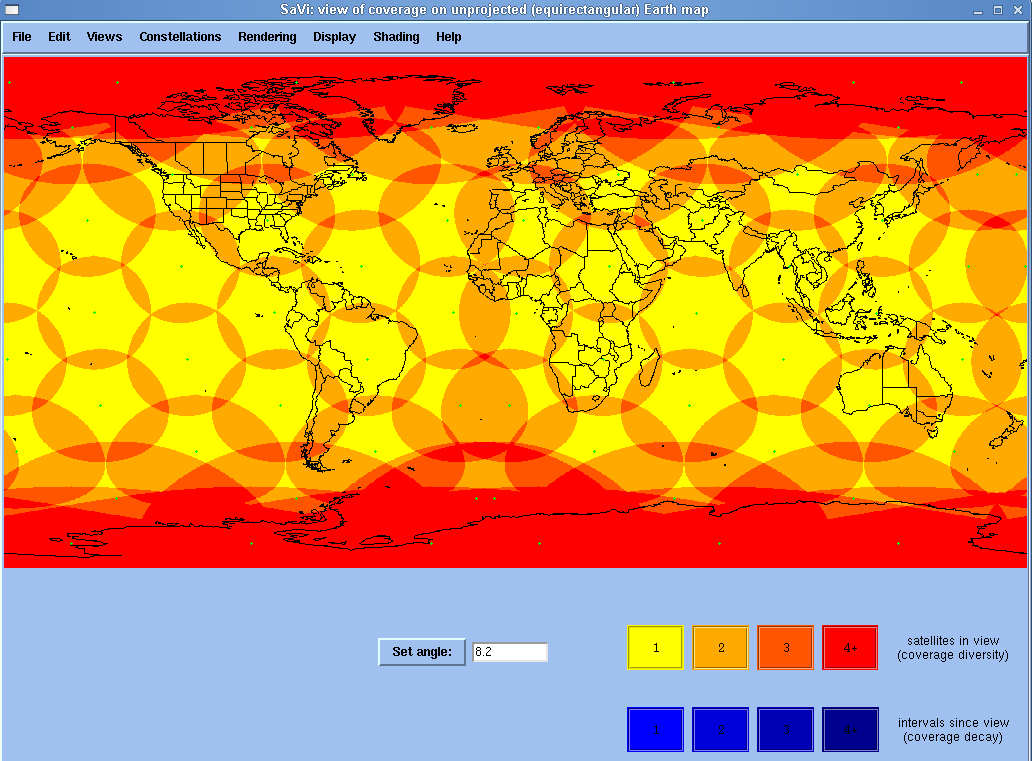
\includegraphics[width=\linewidth, height= 7.6 cm]{Kapitel/Iridium/Grafiken/netzabdeckung82.png}
	\captionof{figure}{Netzabdeckung unter dem Höhenwinkel von 8.2 Grad~\cite{I4}}
	\label{na8.2}
\end{Figure}

\newpage
